\documentclass[a4paper]{article}

\usepackage[english]{babel}
\usepackage[utf8x]{inputenc}
\usepackage[T1]{fontenc}
\usepackage[a4paper,top=3cm,bottom=2cm,left=3cm,right=3cm,marginparwidth=1.75cm]{geometry}
\usepackage{graphicx}
\usepackage{wrapfig}
\usepackage[colorlinks=true, allcolors=blue]{hyperref}

\title{Pick Up! USSA}
\author{Michael Chan (chanmic), Ryan Miura (miurary), \\Christopher Cooper (cooperchri), Jordan Clark (clarkj3), Ziyu Xiong (xiongz)}

\begin{document}
\maketitle

\section{User Stories}
\begin{enumerate}

\item Users will have to option to either create an account or log in to an existing account.
\begin{enumerate}
\item On the homepage of the website, the user will be given two options, Login with an existing account or create an account.
\end{enumerate}

\item Users can create account.
\begin{enumerate}

\item If the user does not have an account, they can select the create an account option. When creating an account, users will create a username and password, re-enter the password to check that it was entered correctly, and provide a valid email for the account. If the username has not been used and all the information was provided the account will be made.
\end{enumerate}

\item Users can validate their account.
\begin{enumerate}
\item Once a user creates an account they will be sent an email to make sure they are a valid user and the account made was not a fake account. The users can check their email and click on the link to validate their email and account. Once the account has been validated the user will be allowed to log in on the homepage of the website with their account information.
\end{enumerate}

\item Users can log in.
\begin{enumerate}
\item Once a user creates an account they will be sent an email to make sure they are a valid user and the account made was not a fake account. The users can check their email and click on the link to validate their email and account. Once the account has been validated the user will be allowed to log in on the homepage of the website with their account information.
\end{enumerate}

\item Users can reset password.
\begin{enumerate}
\item On the login page, the user will be given the option to reset their pass in the case that they forgot their password. If the user selects this option on the login page they will be sent an email giving them the ability to reset their password.
\end{enumerate}

\item Users can update account profile.
\begin{enumerate}
\item Once a valid user has logged in they will continually have the option in the top right corner of their screen, on all future website pages, to update profile. If selected the user will be brought to a page that allows them to change their username, email, or password. Then the information will be saved an updated.
\end{enumerate}

\item Users can view posted events.
\begin{enumerate}
\item Once a user has logged in with a valid account they will be given a list of sports to select from. When the user clicks on a sport they will then be shown a list of all the post that have been made for upcoming events of that sport. For example, once the user logs in they will be given a list of sports shown as buttons (ie: football, basketball, volleyball) then when the user clicks on the sport (ie: basketball) then the user will be shown all upcoming basketball game events that have been posted.
\end{enumerate}

\item Users can search even post with filters.
\begin{enumerate}
\item Once a user selects the sport they will also have the option to filter the events listed. On a sidebar of the even listings of the selected sports, the user can choose to filter done to options to within a specific zip code, date, time, skill leave etc.
\end{enumerate}

\newpage
\item Users can create an event post.
\begin{enumerate}
\item On the sidebar of the event postings where the filters are listed, users will be given the option to make an event post. For an event post, the user will enter the sport, the date and time, where the event is to reoccur or be a one-time event, zip code of the event, and skill level required for the event. Once all the information has been entered the event will be made and will be seen on the listing of event posts with the username of the user that created the event.    
\end{enumerate}

\item Users can make even post reoccurring.
\begin{enumerate}
\item When making a post users chance choose to have the even be a one-time event or a reoccurring event. If an event a reoccurring, when making the event post the creator will be given the option to have the event reoccur daily, weekly, or monthly. The creator of the event will also be asked to enter in an end date of the event or a date at which the event stops reoccurring.     
\end{enumerate}

\item Users can add other users to friend list.
\begin{enumerate}
\item When a user finds an even post they are interested in on the even listings page they can see who was the creator of the event. The user can add this other user add a friend to be able to communicate better about the event.  
\end{enumerate}

\item Users can accept friends.
\begin{enumerate}
\item If one user attempts to add another user as a friend the second user will be given the option to add the user or decline the request. If the request is accepted the two users will become friends. 
\end{enumerate}

\item Users can send message to other users.
\begin{enumerate}
\item Users that are friends will have the ability to message each other. They can use this message tool to discuss details about even posts. 
\end{enumerate}

\item Users can create group chat for a game event.
\begin{enumerate}
\item The creator of an event that has been posted can create an add friends to a group chat. These other users would be people that have been approved to be a participant in the event. 
\end{enumerate}

\item Users can add other users to group chat.
\begin{enumerate}
\item Users that have created an event posting can add other users that they are friends with to a group chat. This way the creator of an even posting can discuss even details with the group of people they have approved to participate in the event they posted.  
\end{enumerate}

\item Users can edit event posts.
\begin{enumerate}
\item Users that have created an event post can go back and edit the post to change the details and information of the post. This will allow users to make the even reoccurring, change the reoccurring date, change the date, time, location and other event details of the event if needed.
\end{enumerate}

\item Users can give other users editing permission to an event.
\begin{enumerate}
\item Users that have made an event post and have to ability to add users to a group chat for the event can give other users admin permission. If another user is given admin permission of a group chat they can also add a user to the group. All other users in the group just have viewing permissions of the group chat.
\end{enumerate}

\end{enumerate}
\newpage

\section{Corresponding Tasks}
For the amount of time each task would take, we denoted it using units of time, u. 0u represents a task that is not complex and therefore would take very little time. 1u represents approximately an hour of effort.
\begin{enumerate}

\item Users can log in with their username/password - first week
\begin{enumerate}
\item Make log-in page - 1u
\item Add server code for username/password hashing/verification - 2u
\end{enumerate}

\item Users can create an account - first week
\begin{enumerate}
\item Make account creation modal - 1u
\item Format database for users - 0u
\item Add server code for storing of account information - 2u
\end{enumerate}

\item Users can create an event post - first week
\begin{enumerate}
\item Make post creation modal - 1u
\item Format database for posts - 0u
\item Add server code to store post information - 2u
\end{enumerate}

\item Users can view event posts - first week
\begin{enumerate}
\item Make post page  - 1u
\item Add server code to fetch/display posts - 1u
\end{enumerate}

\item Users can filter events - first week
\begin{enumerate}
\item Make sidebar filter - 1u
\item Add server code to search/filter posts - 1u
\end{enumerate}

\item Users can edit their existing events - first week
\begin{enumerate}
\item Add server code to fetch/store post information - 1u
\end{enumerate}

\item Users have the choice of logging in or creating an account - first week
\begin{enumerate}
\item Make buttons for log-in/sign-up - 0u
\end{enumerate}

\item Users can make an event recurring - first week
\begin{enumerate}
\item Add dropdown to event creation - 0u
\item Add server code to repeat an event - 1u
\item Add repeated event to database - 0u
\end{enumerate}

\item Users can send a message to another user - second week
\begin{enumerate}
\item Make messages page - 1u
\item Format database for messages - 0u
\item Add server code to fetch/store/send messages between users - 3u
\end{enumerate}

\item Users can add other users to their friends list - second week
\begin{enumerate}
\item Make friends list modal - 1u
\item Format database for friends - 0u
\item Add server code to fetch friends - 2u
\end{enumerate}

\item Users can update their account settings - second week
\begin{enumerate}
\item Make account settings page - 1u
\end{enumerate}

\item Users can add other users to group chats - if time allows
\begin{enumerate}
\item Add server code to send single messages to multiple people - 1u
\end{enumerate}

\item Users can create a group chat for their created events - if time allows
\begin{enumerate}
\item Add button on user’s own events - 0u
\end{enumerate}

\item Users can recover their password by email - if time allows
\begin{enumerate}
\item Add server code to send email with link to page to reset password - 1u
\end{enumerate}

\item Users can validate their account - if time allows
\begin{enumerate}
\item Format database to hold a validated flag - 1u
\item Add server code to send verification email - 1u
\end{enumerate}


\item Users can give additional users editing permissions - if time allows
\begin{enumerate}
\item Format database for edit permissions - 0u
\item Add server code to add users to the post editors database - 1u
\end{enumerate}

\end{enumerate}
\newpage

\section{UML Sequence Diagrams}

First user story: Users can login with a username and password.

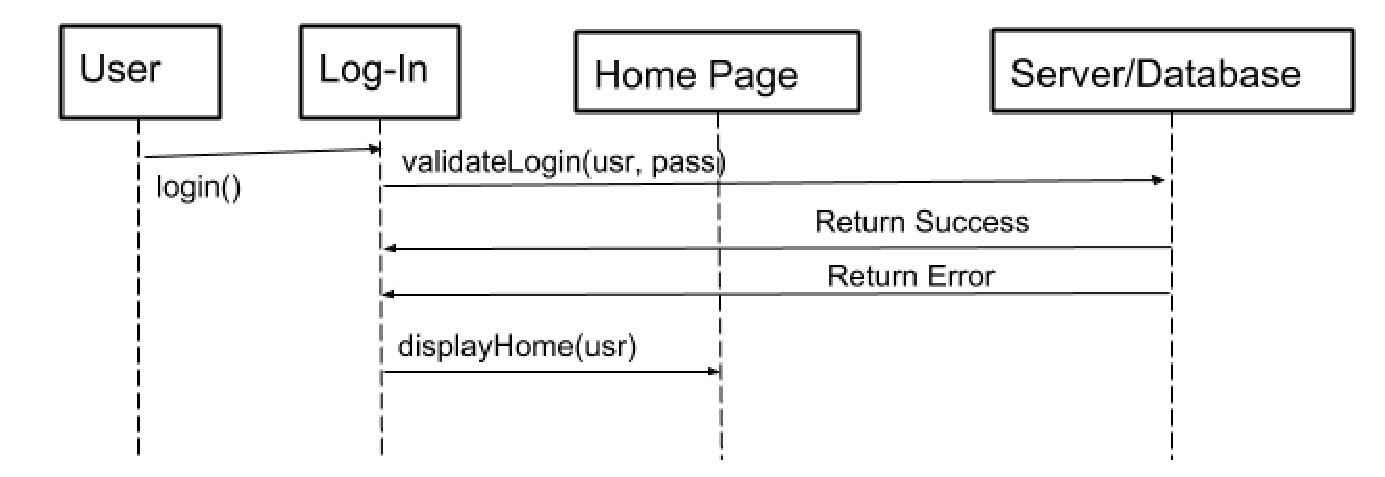
\includegraphics[width=\textwidth]{login}

Second user story: Users can create an account with a username, password, and email.

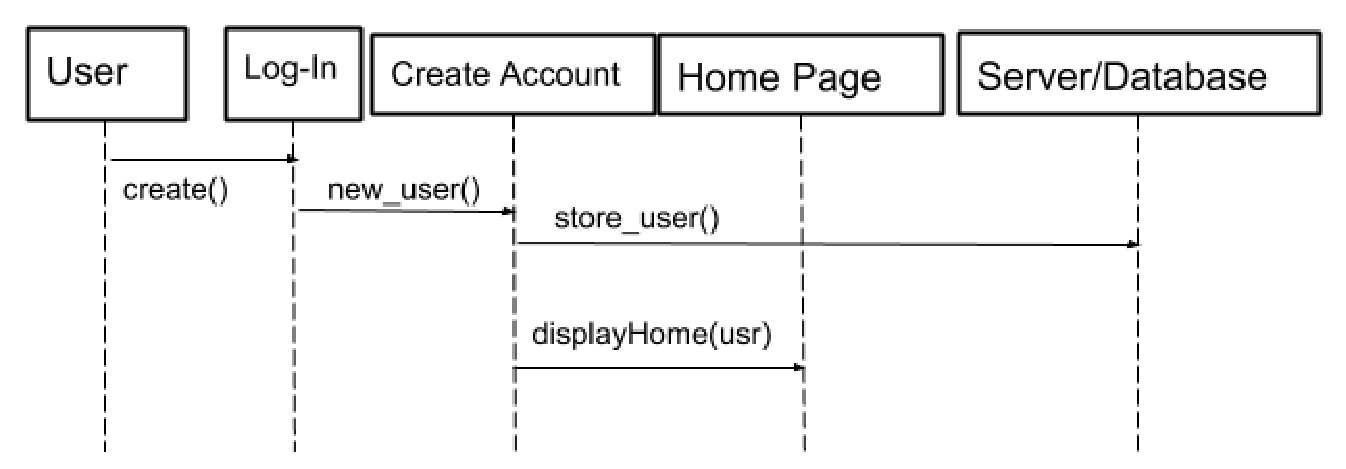
\includegraphics[width=\textwidth]{createAccount}

Third user story: Users can view sport events posts created by users.

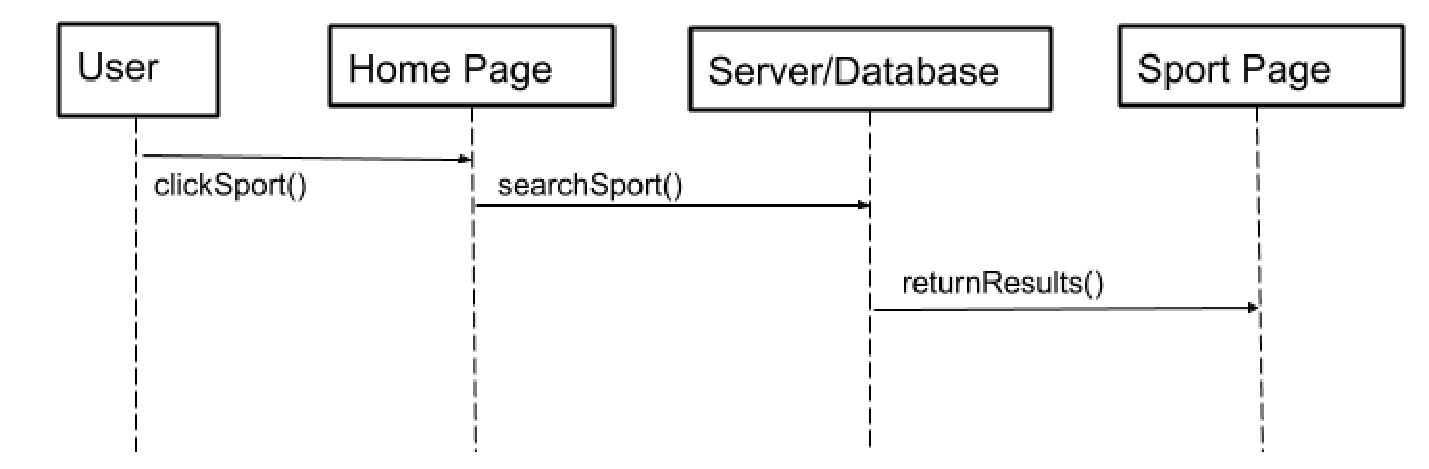
\includegraphics[width=\textwidth]{viewSport}

Fourth user story: Users can create an event post to be stored in the database.

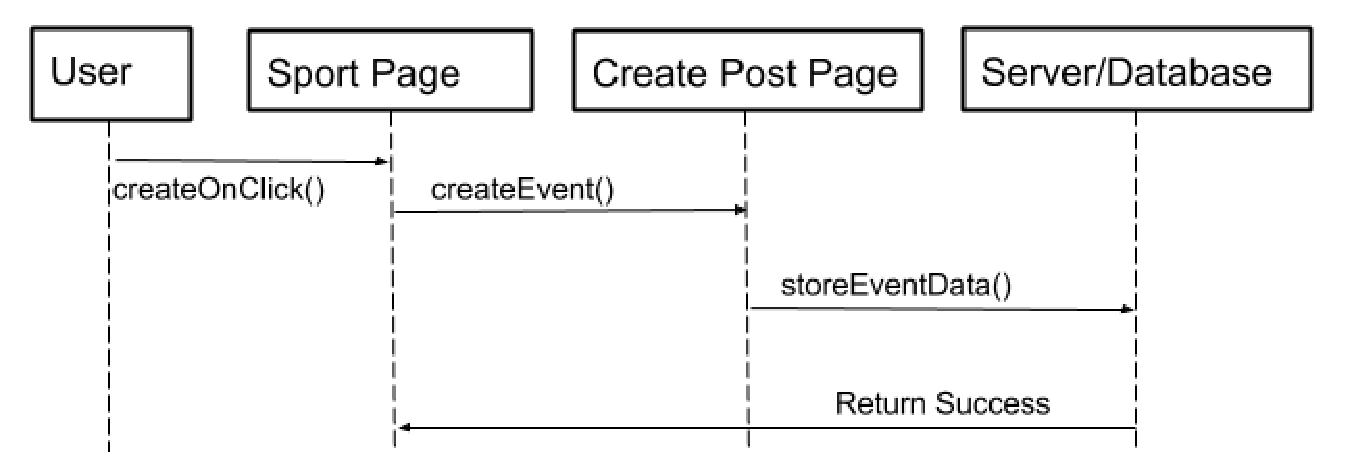
\includegraphics[width=\textwidth]{createEvent}

Fifth user story: Users can edit their event posts.

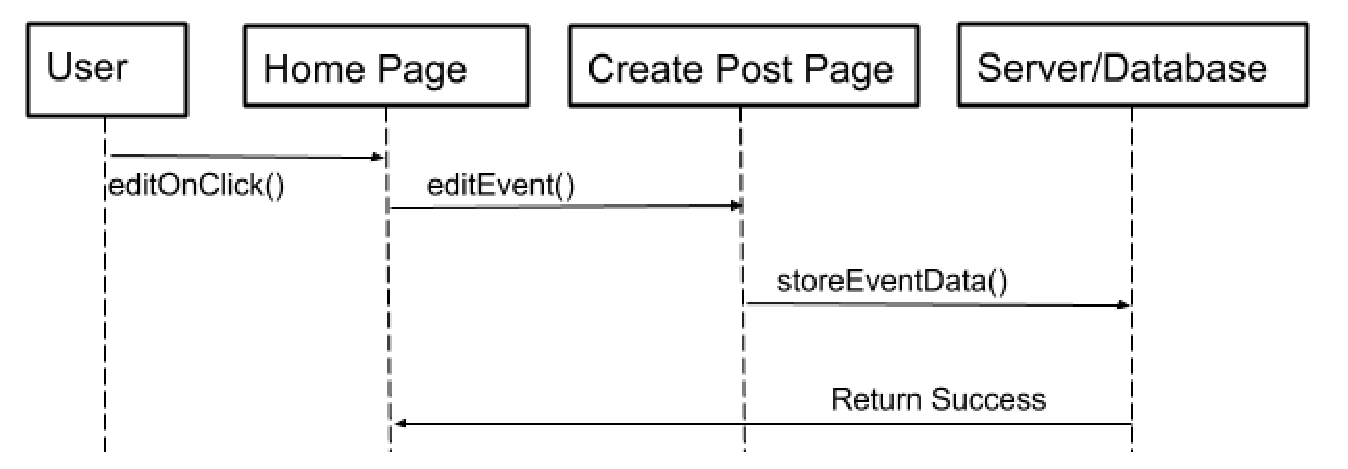
\includegraphics[width=\textwidth]{editEvent}

Sixth user story: Users can filter search results of event posts.

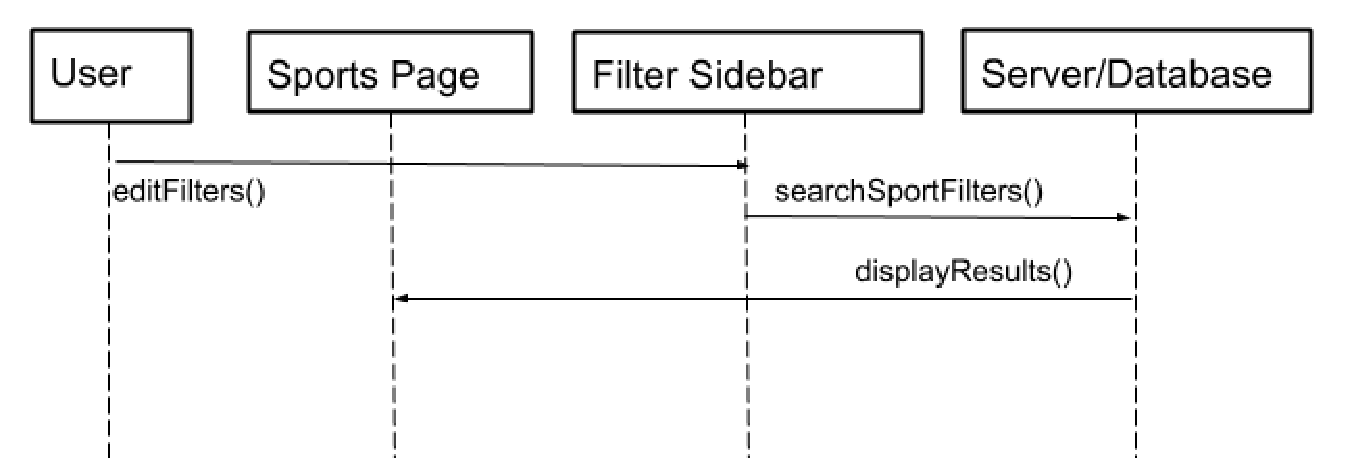
\includegraphics[width=\textwidth]{filter}

Seventh user story: Users can add reoccurence to created event posts.

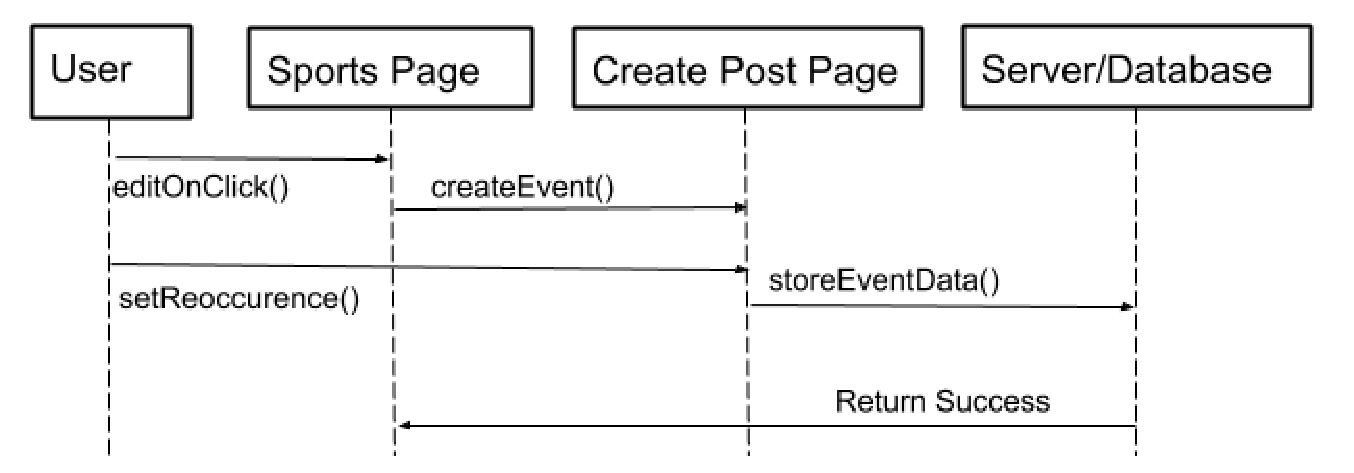
\includegraphics[width=\textwidth]{reoccurence}

\newpage

\section{The Stories Due Next Week}
We decided that six stories will be due next week:
\begin{enumerate}
\item \textbf{Users will be able to log in with a username and password:}
\begin{itemize}
\item In order to finish the user login, a log-in page is needed. 
\item The HTML of the login page will be completed by Ziyu and Cooper. This should be done by March 2nd.
\item Jordan will work on the CSS prototype and finish by March 5th. 
\item Ryan and Michael will be in charge of server-side code in Node.js and its packages and Javascript and finish by March 5th.
\end{itemize}
\item \textbf{Users will be able to create an account with a username, password, and email:}
\begin{itemize}
\item To create an account, a modal will open.
\item Ziyu and Cooper will work on the HTML of the modal and finish by March 2nd.
\item Jordan will work on the CSS prototype and finish by March 5th.
\item Ryan and Michael will work on Node.js and Javascript and finish by March 5th.
\end{itemize}
\item \textbf{Users will be able to create an event post:}
\begin{itemize}
\item To create a post, a modal will open.
\item Ziyu and Cooper will work on the HTML of the modal and finish by March 4th.
\item Jordan will work on the CSS prototype and finish by March 5th.
\item Ryan and Michael will work on Node.js and Javascript and finish by March 5th.
\end{itemize}
\item \textbf{Users will be able to view event posts:}
\begin{itemize}
\item To view posts, a homepage is needed.
\item Ziyu and Cooper will work on the HTML of the homepage and finish by March 4th.
\item Jordan will work on the CSS prototype and finish by March 5th.
\item Ryan and Michael will work on Node.js and Javascript and finish by March 5th.
\end{itemize}
\item \textbf{Users will be able to filter event posts:}
\begin{itemize}
\item To filter posts, a sidebar will be on the side of the homepage.
\item Ziyu and Cooper will work on the HTML of the sidebar and finish by March 4th.
\item Jordan will work on the CSS prototype and finish by March 5th.
\item Ryan and Michael will work on Javascript and finish by March 5th.
\end{itemize}
\item \textbf{Users will be able to edit existing event posts:}
\begin{itemize}
\item To edit a post, a modal will open when a button is pressed.
\item Ziyu and Cooper will work on the HTML of the button and modal and finish by March 4th.
\item Jordan will work on the CSS prototype and finish by March 5th.
\item Ryan and Michael will work on Node.js and Javascript and finish by March 5th.
\end{itemize}
\end{enumerate}
\newpage

\section{Meeting Report}
This week we met in the library for a couple hours. The first part of our meeting was a briefly review of our project in order to confirm the details in the design of user interface and figure out how the database connect to our system. 
Then, we moved to the “user stories” part. At the very beginning, we could only list 9 user stories in our project. Later, we found some of the user stories we made were too general, so we divide these general user stories into many sub-stories which were much more specific and detailed. After finishing all the user stories, we sorted these stories by priority and decide which parts would we do on next week. 

Next week, we will start to work on the coding stuff. In the first implementation assignment, we are planning to work on the “Login Page” and “Sports Page”. We divided our first implementation into 3 parts which are HTML, CSS \& DATABASE. Ziyu and Cooper is going to work on the HTML. Jordan will work on the CSS to design our website. Michael and Ryan will work on the database. And the goal for this assignment is to run our “Login Page” and “Sports Page” successfully. 

Our customers were able to meet with group. One of our customers was my friend who was a student major in Marketing, I briefly introduced our project to her and explained our user stories. Except some of the technical information like the server side, she could mostly catch our points and clearly know how to work on this project. I think this is really a good new to our team, because users can feel comfortable of using our project, even they don’t have any background of CS. There was another customer who is a graduate student and majors in CS in OSU. He said the purpose and the design of the project was clear, not that complicated and he also mentioned the sever side was a critical part in this project. 
According to the responses of these two customers, I think it is reasonable for our project, which include the user with CS background and non-CS background. 

\end{document}